\chapter{A glimpse on advanced topics}


\section{Advanced Bash/Python Scripting}

Here we will cover a few more advanced topics not covered on our introductory scripting session. The examples here are oriented to usual operations that need to be done with the text output from several research codes.

\subsection{Extracting text from output files (awk and grep)}

Consider the data at \verb|Day3_AdvancedTopics/1.Scripting|.
There is a compressed file called \texttt{goldnano3cu.tgz}.
Uncompress the tar file with

\begin{lstlisting}
tar -zxvf goldnano3cu.tgz
\end{lstlisting}

The folders and files are from actual simulations of gold nanoclusters. You can see a sample from the first 10 simulations. The actual simulation was done with actually several hundred files like those.

First, have a look to one of those files. For example \texttt{goldnano3cu/0/output.log}. Use \texttt{less} or your favorite text editor to get an idea about how the file actually looks. With less you can search for words typing \verb|/| and the pattern. Search for etot on that file.

The first challenge is to know the value of the total energy per atom. You can see that such information is contained on lines such as 

\begin{lstlisting}
Time step =    232 SCF step =   3 etot/atom =    -277.072096
\end{lstlisting}

So you can use grep to extract those lines from the output

\begin{lstlisting}
grep "etot/atom" goldnano3cu/0/output.log
\end{lstlisting}

grep is a tool to extract lines from text output using patterns to identify the lines that we need to be shown.

The output will look like this

\begin{lstlisting}
...
   Time step =    251 SCF step =   3 etot/atom =    -277.070767
   Time step =    252 SCF step =   3 etot/atom =    -277.070811
   Time step =    253 SCF step =   3 etot/atom =    -277.070817
   Time step =    254 SCF step =   4 etot/atom =    -277.070855
   Time step =    255 SCF step =   3 etot/atom =    -277.070890
   Time step =    256 SCF step =   3 etot/atom =    -277.070922
   Time step =    257 SCF step =   3 etot/atom =    -277.070953
   Time step =    258 SCF step =   3 etot/atom =    -277.070978
\end{lstlisting}

You can see the file again and noticing that after that line there are more information that could be interesting to see.
Execute for example:

\begin{lstlisting}
grep -A 9 "etot/atom" goldnano3cu/0/output.log
\end{lstlisting}

Now, we are capturing the lines with \verb|'etot/atom'| and the next 9 lines AFTER. You can also use \texttt{-B} to get lines before the pattern.

\begin{lstlisting}
grep -B 1 -A 9 "etot/atom" goldnano3cu/0/output.log
\end{lstlisting}

The pattern so far is just a fixed string. grep was created to use far more complex patterns called regular expressions.

Consider for example that we are searching for lines with the word "Time"

\begin{lstlisting}
grep "Time" goldnano3cu/0/output.log
\end{lstlisting}

But, now we realize that we do not want those lines that start with EBS, so we can indicate grep that the pattern matches only the word "Time" at the beggining of the line with some arbitrary number of spaces.

\begin{lstlisting}
grep "^ *Time" goldnano3cu/0/output.log
\end{lstlisting}

The following list shows the basic elements for regular expressions.

\begin{lstlisting}
. (dot) - a single character.
?       - the preceding character matches 0 or 1 times only.
*       - the preceding character matches 0 or more times.
+       - the preceding character matches 1 or more times.
{n}     - the preceding character matches exactly n times.
{n,m}   - the preceding character matches at least n times        
          and not more than m times.
[agd]   - the character is one of those included 
          within the square brackets.
[^agd]  - the character is not one of those included 
          within the square brackets.
[c-f]   - the dash within the square brackets operates 
          as a range. In this case it means either the 
          letters c, d, e or f.
()      - allows us to group several characters to behave 
          as one.
|       - the logical OR operation.
^       - matches the beginning of the line.
$       - matches the end of the line.
\end{lstlisting}

Regular expressions is whole subject by itself and widely used not only by grep, but also many other languages such as awk, perl and python. We will continue the exploration using AWK.

AWK is a programming language designed for text processing and typically used as a data extraction and reporting tool.
In the 1990s, Perl became very popular, competing with AWK in the niche of Unix text-processing languages. Nowadays is Python the most popular language for many purposes including text processing, however for some basic operations is far easier to use a awk line or small script rather than a python one.

Lets go back to our grep command for extracting the \verb|'etot/atom'|, lets use for example a line like this:

\begin{lstlisting}
grep "^ *Time" goldnano3cu/0/output.log
\end{lstlisting}

Lets suppose that we would like to get just the number of the iteration and the energy, for example to plot the two columns later on. You can use grep and awk connected with a pipe to produce the result. For example

\begin{lstlisting}
grep "^ *Time" goldnano3cu/0/output.log | awk '{print $4, $11}'
\end{lstlisting}

What we are doing here is letting grep to extract the lines that we want and using awk to just print the 4th and 11th column from those lines. Notice the \verb|","| after \verb|$4| otherwise the two numbers will be stick together.

This is a very popular combination, using grep for line extraction and awk to print the output needed.

AWK is able to reproduce the grep execution by itself, for example:

\begin{lstlisting}
awk '(/etot\/atom/) {print $0}' goldnano3cu/0/output.log 
\end{lstlisting}

And the extraction of the iteration number and energy can be done with:

\begin{lstlisting}
awk '(/etot\/atom/) {print $4, $11}' goldnano3cu/0/output.log 
\end{lstlisting}

One of the advantages of AWK is that variables are converted on the fly based on use. That allow us to change the value of the energy if we need for example converted to different units. For example:

\begin{lstlisting}
awk '(/etot\/atom/) {n=$11; print n*0.0367493, "Ha"}' goldnano3cu/0/output.log
\end{lstlisting}

This line also shows how you can create variables and use it them to manipulate the output.

At this point is good to see AWK as an old fashioned C-like scripting language. Take for example this script:

\lstinputlisting[language=C]{../Day3_AdvancedTopics/1.Scripting/awk_squares_cubes.awk}

Lets go back to the output of the simulation. Imagine now that you would like to know the minimum, maximum and average energy per atom. The next script in AWK will do that:

\lstinputlisting[language=C]{../Day3_AdvancedTopics/1.Scripting/awk_min_max_avg.awk}

You can use it like this:

\begin{lstlisting}
awk -f awk_min_max_avg.awk goldnano3cu/0/output.log
\end{lstlisting}

In fact you can go further and process all the outputs from the 10 simulations like this:

\begin{lstlisting}
awk -f awk_min_max_avg.awk goldnano3cu/*/output.log
\end{lstlisting}

AWK is actually reading more than 7 million lines of output, extracting the relevant lines and computing the maximum, minimum and average from them.




\subsection{Regular Expressions with python}

Consider the following challenge.
We have the output from a simulation with some data that we would like to process, the problem now is that the data is not on a single like, so a simple grep will not work. The data we want to parse looks like this:

\begin{lstlisting}
...
     14       7.7300      0.00000
     15       7.9145      0.00000
     16       8.7421      0.00000

 k-point 115 :       0.4444    0.3636    0.4286
  band No.  band energies     occupation 
      1      -6.7076      1.00000
      2      -6.6256      1.00000
      3      -3.8932      1.00000
      4      -3.8031      1.00000
      5       0.1344      1.00000
      6       0.4871      1.00000
      7       0.7520      1.00000
      8       1.1131      1.00000
      9       3.2272      1.00000
     10       3.3574      1.00000
     11       7.4689      0.00000
     12       7.4905      0.00000
     13       7.7325      0.00000
     14       7.9343      0.00000
     15       8.3742      0.00000
     16       8.7648      0.00000

 k-point 116 :       0.0000    0.4545    0.4286
  band No.  band energies     occupation 
      1      -7.0118      1.00000
      2      -6.8668      1.00000
      3      -4.4179      1.00000
...
\end{lstlisting}

This is quite complex set of data and we would like to take the different elements in such a way that we can manipulate them later on.

There are several ways of solving this problem, for example, knowing that each block of data starts with "k-point"
 and spans 17 rows. Such task could be done using just grep
 
\begin{lstlisting}
grep -A 17 k-point OUTCAR 
\end{lstlisting}

The argument "-A 17" will tell grep to show 17 rows after each occurrence of the line k-point.
We extract the line of information that we need but still is just a piece of text that is not so simple to manipulate.

With python we can achieve this task with just 4 lines, using the so called regular expressions, a way to explain a computer that we want extract text with some format by indicating the kind of data that we expect on the text.

This following script will extract the pieces still as text but, we will work on the conversion to text later.

\begin{lstlisting}[language=Python, numbers=left]
import re
rf = open('OUTCAR')
data = rf.read()
kp = re.findall('k-point([\d\s]*):([\d\s.]*)band[\.\s\w]*occupation([\s\d:\-\.]*)\n\n', data)
\end{lstlisting}

The most cryptic part of this small script is understanding the meaning of all those symbols used as arguments for the findall function.
Lets start with a simpler version of the findall line an we will understand it piece by piece.

Using IPython lets start with executing the first 3 lines and we will explore the findall function step by step

\begin{lstlisting}[language=Python, numbers=left]
import re
rf = open('OUTCAR')
data = rf.read()
\end{lstlisting}

Now, we start exploring this line

\begin{lstlisting}[language=Python, numbers=left]
re.findall('k-point[\d\s]*:', data)
\end{lstlisting}

The output will look like this:

\begin{lstlisting}[language=Python, numbers=left]
['k-point  1 :',
 'k-point  2 :',
 'k-point  3 :',
 'k-point  4 :',
\end{lstlisting}

The line in findall can be read like this: Search for text that start with ``k-point" followed by 0 or more (that is the meaning of '*') groups of characters (what is enclose by ``[" and ``]") that can be either numbers "\verb|\d|" or characters that looks like spaces ``\verb|\s|"

Now, if we just need the number, we can enclose the information that findall will return by enclosing it in parenthesis, like this:

\begin{lstlisting}[language=Python, numbers=left]
re.findall('k-point([\d\s]*):', data)
\end{lstlisting}

At this point could be interesting to show how we can convert the list of strings returned by findall into actual numbers.
This could be done like this:

\begin{lstlisting}[language=Python, numbers=left]
[int(x) for x in re.findall('k-point([\d\s]*):', data)]
\end{lstlisting}

Now lets move forward and get the next piece of information, the three numbers after colon, the numbers before the word 'band'

\begin{lstlisting}[language=Python, numbers=left]
re.findall('k-point([\d\s]*):([\d\s.]*)band', data)
\end{lstlisting}

As you can see we are getting more information this time

\begin{lstlisting}
[('   1 ', '       0.0000    0.0000    0.0000\n  '),
 ('   2 ', '       0.1111    0.0000    0.0000\n  '),
 ('   3 ', '       0.2222    0.0000    0.0000\n  '),
 ('   4 ', '       0.3333    0.0000    0.0000\n  '),
 ('   5 ', '       0.4444    0.0000    0.0000\n  '),
 ('   6 ', '       0.0000    0.0909    0.0000\n  '),
 ('   7 ', '       0.1111    0.0909    0.0000\n  '),
 ('   8 ', '       0.2222    0.0909    0.0000\n  '),
...
\end{lstlisting}

The output is a list of tuples, each tuple consisting of two strings. There is just one extra character on the regular expression, dot ``." is added to cover the existence of that character in the 3 numbers after colon. In regular expressions "dot" is used to match any character except a newline. Inside the ``[]" special characters lose their special meaning, so ``dot" here means just a ``.".

Now we can go to our final version of the findall function

\begin{lstlisting}
re.findall('k-point([\d\s]*):([\d\s.]*)band[\s\w.]*occupation([\s\d:.\-]*)\n\n', data)
\end{lstlisting}

The meaning of all this cryptic code become far more clear now, the only notice here is that the character minus ``-" needs still to be escaped like ``\verb|\-|" because it has a meaning for ranges inside ``[]". We close the regular expression with a double \verb|\n\n|, indicating that each block is separated by a double newline.

Out final task is to convert the output from findall into actual numbers such that we can manipulate them for whatever purpose we need.

Lets do first a more simple exercise by storing correctly the k-point number and the three numbers after colon, they are the positions but their actual meaning is not important here.

\begin{lstlisting}[language=Python, numbers=left]
ret=[]
for ikp in kp:
    entry={}
    entry['number']= int(ikp[0])
    entry['position']= [float(x) for x in ikp[1].split()]
    entry['values']= len(ikp[2].split())
    ret.append(entry)
\end{lstlisting}

What we are doing here is creating a list called \textbf{ret}
and for each element in our list kp we will create a python dictionary, converting the elements from the tuple into numbers, the first one will be integer, the second one is a set of three floating point numbers and for the third one we will just split the string into words and count the elements.

\begin{lstlisting}
[{'number': 1, 'position': [0.0, 0.0, 0.0], 'values': 48},
 {'number': 2, 'position': [0.1111, 0.0, 0.0], 'values': 48},
 {'number': 3, 'position': [0.2222, 0.0, 0.0], 'values': 48},
 {'number': 4, 'position': [0.3333, 0.0, 0.0], 'values': 48},
 {'number': 5, 'position': [0.4444, 0.0, 0.0], 'values': 48},
 {'number': 6, 'position': [0.0, 0.0909, 0.0], 'values': 48},
...
\end{lstlisting}

For the position we use a list comprehension, a syntactic construct available in some programming languages for creating a list based on existing lists.

The conversion of values is a bit more elaborated. First, notice that the final element contain 49 elements due to a final string with several dashes. We would like to extract the numbers that are really relevant the floating point numbers. Lets consider just the final element from kp

\begin{lstlisting}
In [44]: kp[-1]
Out[44]: 
(' 120 ',
 '       0.4444    0.4545    0.4286\n  ',
 ' \n      1      -6.6226      1.00000\n      2      -6.5937      1.00000\n      3      -3.7536      1.00000\n      4      -3.7218      1.00000\n      5      -0.0498      1.00000\n      6       0.0803      1.00000\n      7       0.5565      1.00000\n      8       0.6896      1.00000\n      9       3.3146      1.00000\n     10       3.3603      1.00000\n     11       7.6585      0.00000\n     12       7.6740      0.00000\n     13       7.9721      0.00000\n     14       8.0356      0.00000\n     15       8.8014      0.00000\n     16       8.9382      0.00000\n\n\n--------------------------------------------------------------------------------------------------------\n')
\end{lstlisting}

Using Numpy we can easily get the information converted ready easily. Consider this line

\begin{lstlisting}
import numpy
np.array(kp[-1][2].split()[:48], dtype=float).reshape(-1,3)
\end{lstlisting}

This line can be readed like this. Take the last element in kp (kp[-1]). Now take the third element of the tuple (kp[-1][2]). Split the string in words and make a list with the first 48 words encountered

\begin{lstlisting}
kp[-1][2].split()[:48]
\end{lstlisting}

The final step is to convert those 48 strings into numbers as floating point numbers and reshape the whole array in 3 columns.

The final version of this part of the script will look like this:

\begin{lstlisting}
ret=[]
for ikp in kp:
    entry={}
    entry['number']= int(ikp[0])
    entry['position']= [float(x) for x in ikp[1].split()]
    entry['values']= np.array(ikp[2].split()[:48], dtype=float).reshape(-1,3)
    ret.append(entry)
\end{lstlisting}

For reasons that will become clearer later we would like to keep everything as simple lists of numbers rather than numpy arrays. So we will serialize the numpy array into a list of lists

\begin{lstlisting}
ret=[]
for ikp in kp:
    entry={}
    entry['number']= int(ikp[0])
    entry['position']= [float(x) for x in ikp[1].split()]
    entry['values']= np.array(ikp[2].split()[:48], dtype=float).reshape(-1,3).tolist()
    ret.append(entry)
\end{lstlisting}

It is time for us to save the data that we parse in something that allow us to recover later. There are several ways to store python objects into files. One way is using JSON, another is using pickle

Right now, the variable ret is a list of dictionaries where each of them contains either single numbers, lists or lists of lists. We can store that in a JSON file such that we can recover that information easily.

JSON is a lightweight data interchange format inspired by JavaScript object literal syntax.
The JSON module in python offers convenient functions to convert simple variables such as list and dictionaries into strings that could be stored in text files such that their contents could be easily retrieved.

Try first executing something like this

\begin{lstlisting}
import json
json.dumps(ret)
\end{lstlisting}

Not easy to read for a human but that long string can be easily understood by a computer to recover the information you stored in it. Try this version for something clearer to read

\begin{lstlisting}
import json
json.dumps(ret, sort_keys=True, indent=4, separators=(',', ': '))
\end{lstlisting}

Lets now store ret into a file and read it again to test we can recover the file.

\begin{lstlisting}
wf = open('k-points.json','w')
dp = json.dump(ret, wf, sort_keys=True, indent=4, separators=(',', ': '))
wf.close()
\end{lstlisting}

Now lets test recovering the data from the file.

\begin{lstlisting}
rf2=open('k-points.json')
json.load(rf2)
\end{lstlisting}

Finally, lets summarize all that we learn with this example.
The whole script will be listed here:

\lstinputlisting[language=Python]{../Day3_AdvancedTopics/1.Scripting/python_re.py}

\section{Programming in C, Fortran and Python}

Learn a new programming language takes time and goes beyond we can pretend here. It is not only the actual knowledge of the syntax and grammar of the language is also an understanding of the expressiveness of each language for describing operations to a computer. There are 3 full featured programming languages in use today for scientific computing. Fortran, C and Python. 

\begin{figure}
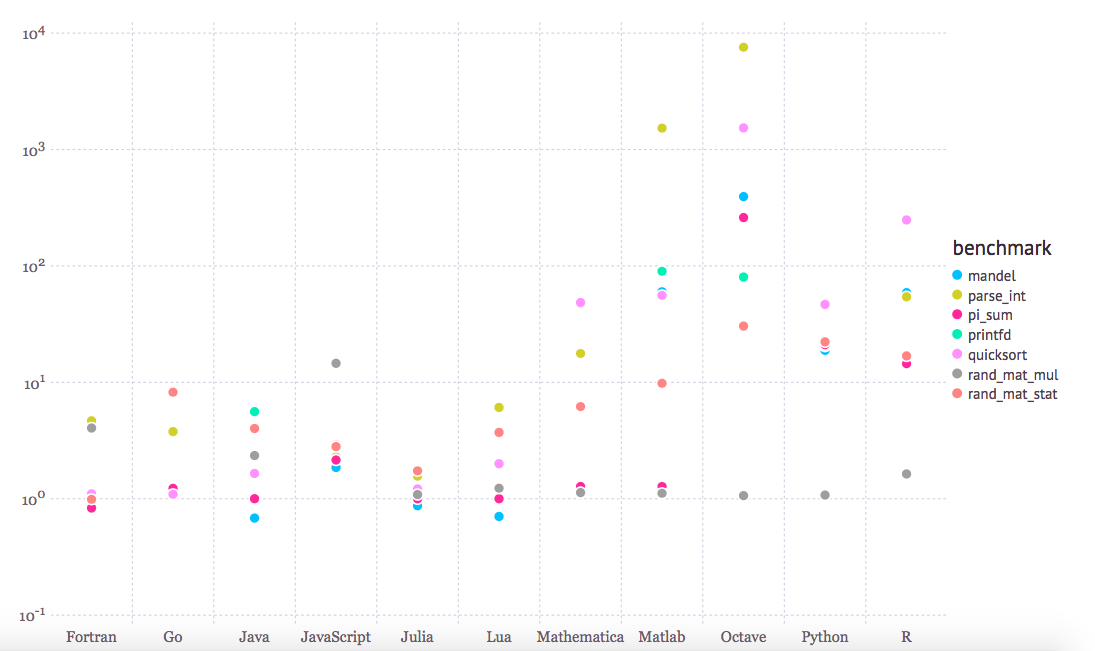
\includegraphics[width=0.95\textwidth]{images/julia_benchmark.png}
\label{bench}
\caption{Comparison of performance for several computing languages. Benchmark times relative to C (smaller is better, C performance = 1.0). Source: https://julialang.org/benchmarks/.}
\end{figure}


There are more specialized languages, such as R, Julia. But we will try to keep the things simple here by showing how the same task is programmed in the 3 languages we have selected.
See for example \ref{bench} for a comparison on the performance of those different languages.

I am taking these examples from http://rosettacode.org.
To give you a flavor of what is the feeling writing code in those 3 languages I have selected 2 tasks and showing how the solution is express in those languages.

\subsection{Sieve of Eratosthenes}

The Sieve of Eratosthenes is a simple algorithm that finds the prime numbers up to a given integer.

Lets start with the implementation in C. I am selecting not the most optimized version, but the simplest implementation for pedagogical purposes. The idea is to get a flavor of the language.

\lstinputlisting[language=C]{../Day3_AdvancedTopics/2.Programming/sieve.c}

This example shows the basic elements from the c language, the creation of variables, loops and conditionals. The inclusion of libraries and the printing on screen.

You can compile this code using the code at 

\begin{lstlisting}
Day3_AdvancedTopics/2.Programming
\end{lstlisting}

\begin{lstlisting}
gcc sieve.c -o sieve
\end{lstlisting}

and execute like this

\begin{lstlisting}
./sieve 100
\end{lstlisting}

Now lets consider the Fortran version of the same problem.

\lstinputlisting[language=Fortran]{../Day3_AdvancedTopics/2.Programming/sieve.f90}

You can notice the particular differences of this language compared with C, working with arrays is in general easier with Fortran.

You can compile this code using the code at 

\begin{lstlisting}
Day3_AdvancedTopics/2.Programming
\end{lstlisting}

\begin{lstlisting}
gfortran sieve.f90 -o sieve
\end{lstlisting}

and execute like this

\begin{lstlisting}
./sieve 100
\end{lstlisting}

Finally, this is the version of the Sieve written in python

\lstinputlisting[language=Fortran]{../Day3_AdvancedTopics/2.Programming/sieve.py}

Python is an interpreted language so you do not need to compile it, instead directly execute the code at:

\begin{lstlisting}
Day3_AdvancedTopics/2.Programming
\end{lstlisting}

using the command line:

\begin{lstlisting}
python sieve.py 100
\end{lstlisting}

\subsection{Matrix inversion}

The purpose here is not to show the algorithm behind matrix inversion but to show how that could be achieve in several programming languages using external libraries, in particular we will show you the problem solved using LAPACK for Fortran, GSL for C and Numpy for python

Lets start with the Fortran version. BLAS and LAPACK are a set of well known libraries to perform Linear Algebra calculations. This is a simple example of inverting a real matrix.


\lstinputlisting[language=Fortran]{../Day3_AdvancedTopics/2.Programming/inverse_matrix.f90}







%\begin{lstlisting}[language=Python, numbers=left]
%import numpy as np
%def incmatrix(genl1,genl2):
%    m = len(genl1)
%    n = len(genl2)
%    M = None #to become the incidence matrix
%    VT = np.zeros((n*m,1), int)  #dummy variable
% 
%    #compute the bitwise xor matrix
%    M1 = bitxormatrix(genl1)
%    M2 = np.triu(bitxormatrix(genl2),1) 
% 
%    for i in range(m-1):
%        for j in range(i+1, m):
%            [r,c] = np.where(M2 == M1[i,j])
%            for k in range(len(r)):
%                VT[(i)*n + r[k]] = 1;
%                VT[(i)*n + c[k]] = 1;
%                VT[(j)*n + r[k]] = 1;
%                VT[(j)*n + c[k]] = 1;
% 
%                if M is None:
%                    M = np.copy(VT)
%                else:
%                    M = np.concatenate((M, VT), 1)
% 
%                VT = np.zeros((n*m,1), int)
% 
%    return M
%\end{lstlisting}


\section{Introduction to Parallel Programming}

Parallel programming is essential in High-Performance Computing. Computers nowadays are not increasing speed as they use to years ago.
Instead, they increase the number of cores.
Modern HPC clusters are now build from several nodes, with several processors each and with several cores each processor.
Those processing capabilities are complemented by adding GPU and Co-processors such as Xeon Phi.

For this tutorial we will consider two popular alternatives for parallel computing, both OpenMP and MPI offers ways of execute calculations concurrently on several cores.
An application can run on a computer cluster using both OpenMP and Message Passing Interface (MPI), such that OpenMP is used for parallelism within a (multi-core) node while MPI is used for parallelism between nodes.

We will explore those two kinds of parallel programming alternatives with a few examples each.

\section{Parallel Programming with OpenMP}

OpenMP (Open Multi-Processing) is an application programming interface (API) that supports multi-platform shared memory multiprocessing programming in C, C++, and Fortran.

The basic idea is to write special comments called ``pragmas" that will be interpreted by the compiler when you compile the code with some special argument. In most cases the code can compile just fine without the extra argument and it will work as a serial code, using just one core.

Lets start with the usual hello program. This is the implementation in C 

\lstinputlisting[language=C]{../Day3_AdvancedTopics/4.OpenMP/omp_hello.c}

You compile it with the command

\begin{lstlisting}
gcc -fopenmp omp_hello.c -o hello
\end{lstlisting}

The version in Fortran is:

\lstinputlisting[language=C]{../Day3_AdvancedTopics/4.OpenMP/omp_hello.f90}

You compile it with the command

\begin{lstlisting}
gcc -fopenmp omp_hello.f90 -o hello
\end{lstlisting}

When you execute the program you will see messages comming from the different threads, all the program runs on the same machine but it creates threads to concurrently execute the section enclosed by the \verb|"#pragma"| or \verb|"!$omp"|
blocks.

You can control the number of threads using

\begin{lstlisting}
export OMP_NUM_THREADS=3
\end{lstlisting}


\section{Parallel Programming with MPI}


\section{Test Driven Development}


\section{Version control with Git}

The tutorial about Git will be based on the repository created at:

\begin{lstlisting}
https://github.com/guilleaf/TutorialGitAutotools
\end{lstlisting}


%\section{Optimization, Profiling and Debugging}

%\section{Creating Python Modules}
%\section{Continuous Integration}
